\documentclass[10pt, a4paper, twocolumn]{article}
%\usepackage{amsmath}
%\usepackage{amssymb}
%\usepackage{algorithm}
\usepackage{float}

%%%%%%%%%%%%%%%%%%%%%%%%%%%%%%%%%%%%%%%%%
% Wenneker Article
% Structure Specification File
% Version 1.0 (28/2/17)
%
% This file originates from:
% http://www.LaTeXTemplates.com
%
% Authors:
% Frits Wenneker
% Vel (vel@LaTeXTemplates.com)
%
% License:
% CC BY-NC-SA 3.0 (http://creativecommons.org/licenses/by-nc-sa/3.0/)
%
%%%%%%%%%%%%%%%%%%%%%%%%%%%%%%%%%%%%%%%%%

%----------------------------------------------------------------------------------------
%	PACKAGES AND OTHER DOCUMENT CONFIGURATIONS
%----------------------------------------------------------------------------------------

\usepackage[english]{babel} % English language hyphenation

\usepackage{microtype} % Better typography

\usepackage{amsmath,amsfonts,amsthm} % Math packages for equations

\usepackage[svgnames]{xcolor} % Enabling colors by their 'svgnames'

\usepackage[hang, small, labelfont=bf, up, textfont=it]{caption} % Custom captions under/above tables and figures

\usepackage{booktabs} % Horizontal rules in tables

\usepackage{lastpage} % Used to determine the number of pages in the document (for "Page X of Total")

\usepackage{graphicx} % Required for adding images

\usepackage{enumitem} % Required for customising lists
\setlist{noitemsep} % Remove spacing between bullet/numbered list elements

\usepackage{sectsty} % Enables custom section titles
\allsectionsfont{\usefont{OT1}{phv}{b}{n}} % Change the font of all section commands (Helvetica)

%----------------------------------------------------------------------------------------
%	MARGINS AND SPACING
%----------------------------------------------------------------------------------------

\usepackage{geometry} % Required for adjusting page dimensions

\geometry{
	top=1cm, % Top margin
	bottom=1.5cm, % Bottom margin
	left=2cm, % Left margin
	right=2cm, % Right margin
	includehead, % Include space for a header
	includefoot, % Include space for a footer
	%showframe, % Uncomment to show how the type block is set on the page
}

\setlength{\columnsep}{7mm} % Column separation width

%----------------------------------------------------------------------------------------
%	FONTS
%----------------------------------------------------------------------------------------

\usepackage[T1]{fontenc} % Output font encoding for international characters
\usepackage[utf8]{inputenc} % Required for inputting international characters

\usepackage{XCharter} % Use the XCharter font

%----------------------------------------------------------------------------------------
%	HEADERS AND FOOTERS
%----------------------------------------------------------------------------------------

\usepackage{fancyhdr} % Needed to define custom headers/footers
\pagestyle{fancy} % Enables the custom headers/footers

\renewcommand{\headrulewidth}{0.0pt} % No header rule
\renewcommand{\footrulewidth}{0.4pt} % Thin footer rule

\renewcommand{\sectionmark}[1]{\markboth{#1}{}} % Removes the section number from the header when \leftmark is used

%\nouppercase\leftmark % Add this to one of the lines below if you want a section title in the header/footer

% Headers
\lhead{} % Left header
\chead{\textit{\thetitle}} % Center header - currently printing the article title
\rhead{} % Right header

% Footers
\lfoot{} % Left footer
\cfoot{} % Center footer
\rfoot{\footnotesize Page \thepage\ of \pageref{LastPage}} % Right footer, "Page 1 of 2"

\fancypagestyle{firstpage}{ % Page style for the first page with the title
	\fancyhf{}
	\renewcommand{\footrulewidth}{0pt} % Suppress footer rule
}

%----------------------------------------------------------------------------------------
%	TITLE SECTION
%----------------------------------------------------------------------------------------

\newcommand{\authorstyle}[1]{{\large\usefont{OT1}{phv}{b}{n}\color{DarkRed}#1}} % Authors style (Helvetica)

\newcommand{\institution}[1]{{\footnotesize\usefont{OT1}{phv}{m}{sl}\color{Black}#1}} % Institutions style (Helvetica)

\usepackage{titling} % Allows custom title configuration

\newcommand{\HorRule}{\color{DarkGoldenrod}\rule{\linewidth}{1pt}} % Defines the gold horizontal rule around the title

\pretitle{
	\vspace{-30pt} % Move the entire title section up
	\HorRule\vspace{10pt} % Horizontal rule before the title
	\fontsize{32}{36}\usefont{OT1}{phv}{b}{n}\selectfont % Helvetica
	\color{DarkRed} % Text colour for the title and author(s)
}

\posttitle{\par\vskip 15pt} % Whitespace under the title

\preauthor{} % Anything that will appear before \author is printed

\postauthor{ % Anything that will appear after \author is printed
	\vspace{10pt} % Space before the rule
	\par\HorRule % Horizontal rule after the title
	\vspace{20pt} % Space after the title section
}

%----------------------------------------------------------------------------------------
%	ABSTRACT
%----------------------------------------------------------------------------------------

\usepackage{lettrine} % Package to accentuate the first letter of the text (lettrine)
\usepackage{fix-cm}	% Fixes the height of the lettrine

\newcommand{\initial}[1]{ % Defines the command and style for the lettrine
	\lettrine[lines=3,findent=4pt,nindent=0pt]{% Lettrine takes up 3 lines, the text to the right of it is indented 4pt and further indenting of lines 2+ is stopped
		\color{DarkGoldenrod}% Lettrine colour
		{#1}% The letter
	}{}%
}

\usepackage{xstring} % Required for string manipulation

\newcommand{\lettrineabstract}[1]{
	\StrLeft{#1}{1}[\firstletter] % Capture the first letter of the abstract for the lettrine
	\initial{\firstletter}\textbf{\StrGobbleLeft{#1}{1}} % Print the abstract with the first letter as a lettrine and the rest in bold
}

%----------------------------------------------------------------------------------------
%	BIBLIOGRAPHY
%----------------------------------------------------------------------------------------

\usepackage[backend=bibtex,style=authoryear,natbib=true]{biblatex} % Use the bibtex backend with the authoryear citation style (which resembles APA)

\addbibresource{example.bib} % The filename of the bibliography

\usepackage[autostyle=true]{csquotes} % Required to generate language-dependent quotes in the bibliography
 % Specifies the document structure and loads requires packages

%----------------------------------------------------------------------------------------
%	ARTICLE INFORMATION
%----------------------------------------------------------------------------------------

\title{A Comparison Between Various AI Models for Blackjack} % The article title

\author{
	\authorstyle{Krystian Wojcicki \textsuperscript{1}} % Authors
	\newline\newline % Space before institutions
	\textsuperscript{1}\institution{Carleton University, 101001444}\\ % Institution 1
}

\date{April 16, 2020} % Add a date here if you would like one to appear underneath the title block, use \today for the current date, leave empty for no date

%----------------------------------------------------------------------------------------

\begin{document}

\maketitle % Print the title

\thispagestyle{firstpage} % Apply the page style for the first page (no headers and footers)

%----------------------------------------------------------------------------------------
%	ABSTRACT
%----------------------------------------------------------------------------------------

\lettrineabstract{In this paper various AI techniques are compared for playing Blackjack, a card game involving a player and a dealer. Blackjack contains both an element of chance as well as imperfect information, with the player unable to see all of the dealers cards. Genetic Algorithms, Fuzzy Logic Genetic Algorithms, Monte-Carlo Simulations and Q-Learning (a type of reinforcement learning) are compared against a baseline strategy which utilizes the true calculated optimal moves. Expected loss is used to compare the different techniques.}

%----------------------------------------------------------------------------------------
%	ARTICLE CONTENTS
%----------------------------------------------------------------------------------------

\section{Problem Domain}
\begin{figure*}
\centerline{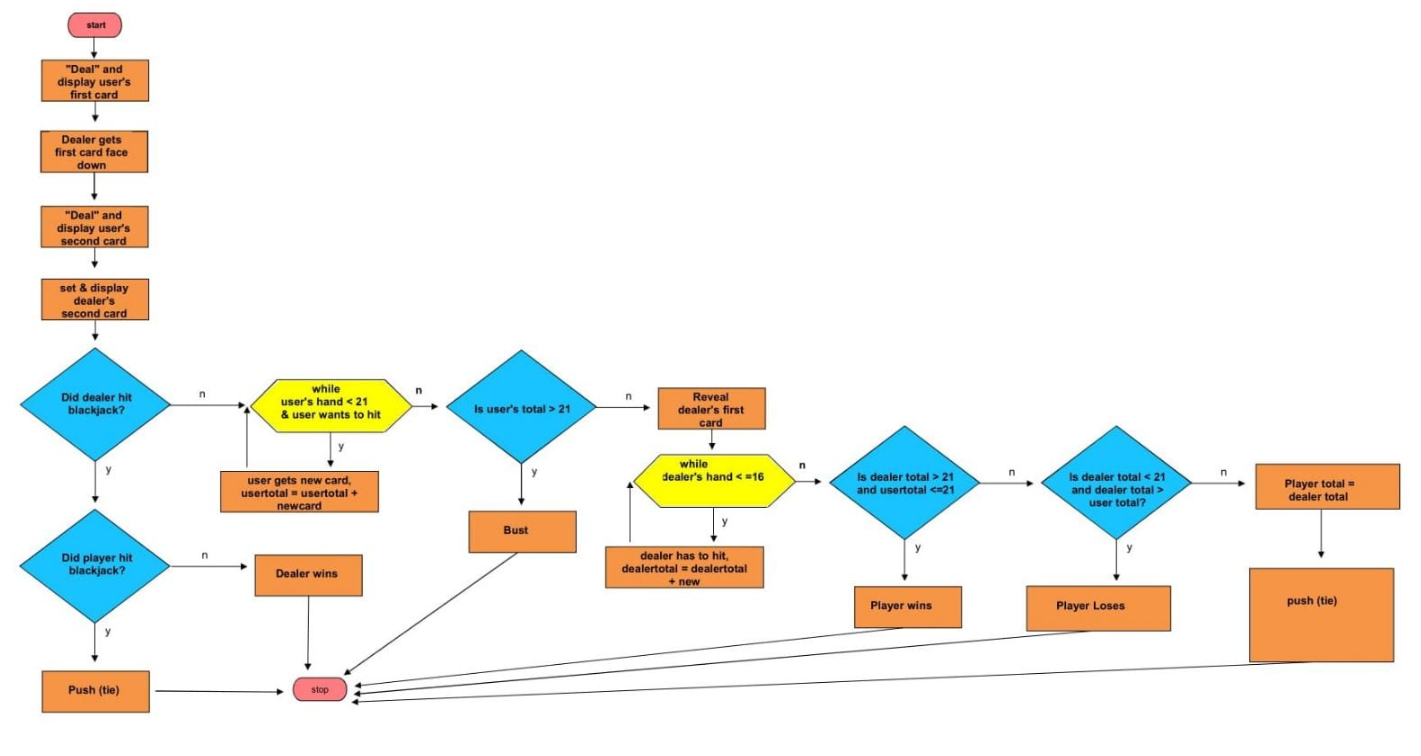
\includegraphics[scale=0.55]{flowchart}}
\caption{Flowchart explaining how the game Blackjack is played}
\label{fig:blackjack}
\end{figure*}
Blackjack, also known as Twenty One, is a card game played between one or more players and a dealer where each player in turn competes against the dealer. Players do not compete against each other and aside from using cards from the same deck, do not impact themselves. 

As can be seen from Figure \ref{fig:blackjack} the rules of the game are not too complex, but still complex enough to not have an obvious strategy. The rules for the dealer are given as a fact so the game can be simulated. 

\section{Motivation}

In class several techniques were taught in how to deal with one and two player games: MiniMax, A*, bfs etc. The problem with these methods was all moves had an equal chance of occurring. In the game of Blackjack depending on the dealers cards and your cards, the probability of of receiving a specific card when "hitting" differs. In addition unlike say in chess or Mancala, there is hidden information. One cannot see the other dealers card. I thought learning how to deal with these uncertainties would be an interesting and challenging problem. 

\section{Proposed Approach}

Several techniques will be compared, Genetic Algorithms (or GA) [1], Fuzzy Logic Genetic Algorithms [7], Monte-Carlo Simulation (MC) [4], Q-Learning [3] against a baseline optimal strategy. 

\subsection{Monte-Carlo Simulation (MC)}

MC have some similarity to the MiniMax algorithm taught in class. In MiniMax all possible moves were generated an evaluated, excluding those ones pruned by alpha/beta. The primary difference being the production system is replaced by a simulation system. Where the simulation system simulates the game and provides simulated outputs. This allows the search to approximate the chance of a certain event happening, without necessarily actually knowing the probability. 

Given any hand with enough simulations the optimal choice between hit and stand can be estimated ie $n := $ \# of simulations, $n \Rightarrow \infty$ then $E(loss)$ is minimized. However there comes a cost of increasing $n$, mainly the speed of the algorithm. With a larger $n$ the time increases exponentially. Unfortunately with an $n$ too small, statistically unlikely (but possible) events are able to sway the simulation and impact the estimated expected loss.

For example if $n = 2, players-total = 20$ and assuming cards are drawn with replacement, to simplify calculations. The optimal move is stand, however there is a $\frac{4}{52} \simeq 7.69\%$ chance of hitting an ace and receiving a total of 21. If one can guarantee an ace then the optimal move is to hit. With $n = 2$ a simulation is likely to hit two aces in a row with a probability of $7.69\%^2 = 0.592\%$. Which is unlikely but with a large enough number of test hands, quite likely to happen causing the expected loss to be incorrectly estimated in some simulations and for a non optimal action to be picked. If $n$ is increased to 5 then the chance of hitting an ace 5 times in a row is $0.000269\%$, essentially never to happen and unlikely to skew any expected loss estimations. As $n$ increases the estimated expected loss moves closer and closer to the actual estimated loss. Without having to deal with calculating the true odds of various events to happen.

\subsection{Genetic Algorithms (GA)}
\begin{figure*}
\centerline{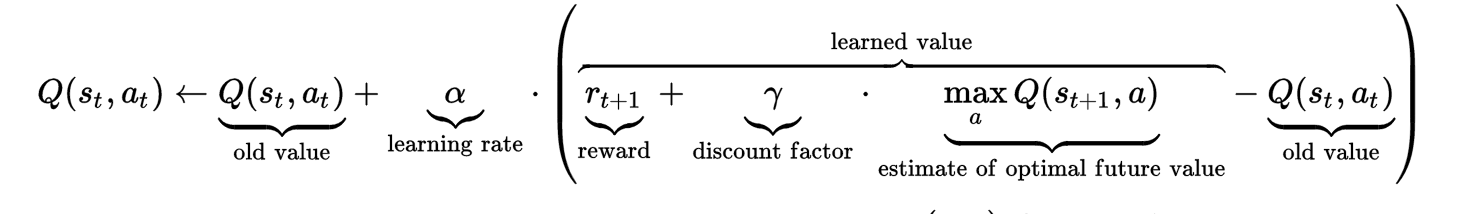
\includegraphics[scale=0.55]{qlearn}}
\caption{Bellman's Equation [2] }
\label{fig:qlearn}
\end{figure*}
GA's function as a search heuristic that utilizes a survival of the fitness technique for obtaining a solution. This technique is often utilized for optimization problems where an optimal solution is not necessary and a near optimal solution is acceptable. First the population is initialized randomly with $k$ chromosomes, each chromosome consists of genes of value $0/1$, indicating whether to hit or stand. Then a cycle of selection, mutation and crossover and done until a stop criteria is met, either a maximum number of iterations or the fitness reaches some maximum.

The selection stage consists of ranking all the chromosomes by a fitness function, in our case the fitness function is the expected loss when using that strategy. 

The top $x$ chromosomes are then taken for breeding and will be referenced to as the mating pool.  For each new solution to be made a pair of parent solutions are selected randomly (from the mating pool), and a crossover procedure is done with the two parents. In addition to  random selection, Roulette Wheel Selection (RWS) [9] was attempted. The name of RWS stems from the fact that here a roulette wheel with slots sized according to the fitness of the individuals used, for example if $F = \sum_{k}{eval(v_k)}$ is the fitness of the mating pool, then the probability of an individual $v_k$ being selected is $p_k = eval(v_k)/F$. RWS allows for all Chromosomes to have a chance to breed, but typically those with higher fitness will breed. This may lead to overfitting or converging to a local minimum however. 

The crossover procedure consists of two steps, first a crossover point is selected as as can be seen in Figure \ref{fig:ga_crossover}. Next all the genes before the crossover point are swapped. For example if two parent Chromosomes exist $A_1 = [x_1, x_2, x_3, x_4], A_2 = [y_1, y_2, y_3, y_4]$ next a random crossover point is selected $c_{rossover} = 2$. Then the first two genes of both the two parent Chromosomes are swapped, resulting in the follow two modified Chromosomes $\alpha_1 = [y_1, y_2, x_3, x_4], \alpha_2 = [x_1, x_2, y_3, y_4]$. 

Then each gene in the new child is mutated with a probability $\alpha$. Once $k$ new chromosomes are created using the previous steps selection begins again. 

The hyper-parameters $k$, $x$ and $\alpha$ are critical parameters that have a high impact on the ability to find better populations. If the mutation probability is too high the new children will essentially be random and the populations average fitness will not increase. If the mutation is probability is too low then the algorithm may converge too early due to a lack of genetic diversity. Having $k$ or $x$ be too small may lead too large variations in fitness or premature convergence again. 


\begin{figure}[H]
\centerline{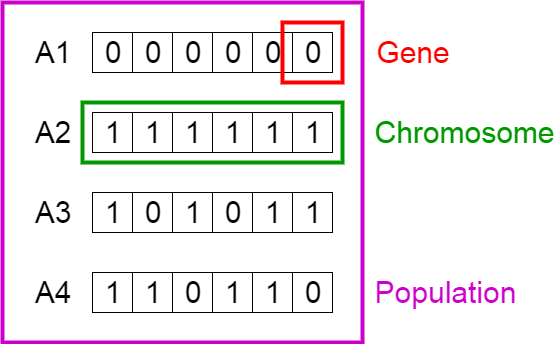
\includegraphics[scale=0.25]{ga_population}}
\caption{Figure depicting the various terms used in Genetic Algorithms. Primarily population which consists of all the Chromosomes, where each Chromosome consists of $w$ Gene's where the value of a Gene specifies which action to be taken in a given state.}
\label{fig:ga_population}
\end{figure}


\begin{figure}[H]
\centerline{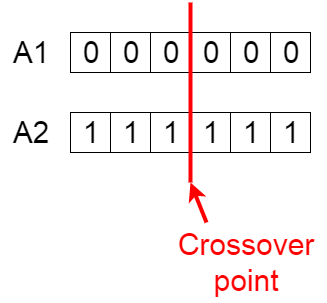
\includegraphics[scale=0.25]{ga_crossover}}
\caption{Figure depecting a random crossover point that is chosen.}
\label{fig:ga_crossover}
\end{figure}

\subsection{Fuzzy Logic Genetic Algorithms (FL-GA)}

Fuzzy Logic attempts to mathematically describe concepts that are vague or open to interpretation. For example it is tough to mathematically describe what the descriptor "warm" means with regards to temperature, as "warm" is different for everyone. Instead to describe "warm" or other descriptors, values are assigned a likelihood that they could qualify for a given descriptor.

For Blackjack this can extended where the membership values are defined for each of the available actions. For example for a given hand the various actions may be given the following probabilities, 10\% to surrender, 50\% to stand, 70\% to hit and 35\% to double down. Note in this paper we do not discuss the possibility of surrendering or being able to double down. Also its important to note that the likelihoods do not have to add up to 100\% as normal probabilities would. In most circumstances for the given hand the most correct answer is to hit, but all options are viable and the player can select any of them. 

This Fuzzy Logic template can be used to modify the previously explained Genetic Algorithms. Instead of one Gene per player's total, there are now two. One which holds the membership for hit and one for standing. When a Fuzzy Logic agent is required to make a decision, the value of the players' hand are used to identify the correct set of values. Then two random doubles between $[0, 1)$ are generated, and each is compared to the value in one of the cells. If the number if less than or equal to the value held by its respective cell the action is suggested. One of the suggested actions is selected at random. If no action is selected a random decision is made. 

The same crossover and mutations are applied to the Chromosomes, the only difference is the mutation instead of generating a random number from the set $\{0, 1\}$, a random number in the range $[0, 1)$ is generated. The hyper-parameters $k$, $x$ and $\alpha$ all have the same meaning in this context. 

In addition to applying the random mutation operator, a Gaussian Mutation Operator was tried out. Since this operators only on floats (or integers if the range of integers is larger than 2) it can only be tried out on the Fuzzy Logic Genetic Algorithm agents. Instead of randomly picking a real number in the range of $[0, 1)$ a random number is picked following the following formula $min(max(N(x, \sigma), a), b)$ where in our case $a = 0, b = 0.99$. 

\subsection{Q-Learning}

The objective in reinforcement learning is to maximize the reward for an agent by taking a series of actions in response to a dynamic environment. A model-free reinforcement learning algorithm is one that estimates the optimal policy without using or estimating the dynamics, transition and reward functions, of the environment. 

Q-Learning is a model free reinforcement learning algorithm to learn a policy telling an agent what action to take under the given circumstances. It does not need to model the environment, which is why this is called a model free algorithm. Q-Learning is values based learning algorithm, value based algorithms update the value function based on an equation (depicated in Figure \ref{fig:qlearn}). Q-Learning is also an off-policy leaner meaning it learns the value of the optimal policy independently of the agents actions. 

The Q in Q-Learning stands for quality, quality here represents how useful a given action is in gaining some future reward. So for a state $s$, if there are two actions $a_1, a_2$ then the one that should be picked is the one with higher quality. Now comes the question how to calculate this quality. We can define $Q^*(s, a)$ as the expected value (cumulative discounted reward) of doing action $a$ when presented with state $s$ where action $a$ is assumed to follow the optimal policy. Q-Learning uses temporal differences to estimate the value of $Q^*(s, a)$. Temporal differences is an agent learning from an environment through episodes with no prior knowledge of the environment. The Q-Learning agent maintains a table of $Q[S, A]$ where S are all possible states and A is the set of all actions permissible.  $Q[s, a]$ represents the agents current estimate of $Q^*(s, a)$. The Quality value is updated according to the formula seen in Figure \ref{fig:qlearn}.

For Q-Learning it is critical to choose a good learning rate. With a learning rate too high the estimates may oscillate never being able to converge to the solution. With a learning rate that is too small the agent may never learn the optimal quality estimates. 

\subsection{Optimal Basic Strategy}

Given Blackjack is a one vs one game with the dealer strategy not varying it is possible to calculate the optimal strategy which minimizes the long term house advantage (which is the same as minimizing the expected loss of the player). 

There are several points which can be taken into account while generating these strategies, for example whether or not to take into account the actual card the dealer has, or simply the point total. The more that is taken into account will allow for a better strategy to be created. As a baseline the basic strategy will be utilized, ie only the point total of the dealer will be taken into account. No card counting/composition dependent strategy will be used for the baseline. 

\begin{table}[H]
	\centering
	\begin{tabular}{lllllllllllr}
		\toprule
		\multicolumn{11}{c}{Dealer's face-up card} \\
%		\cmidrule(r){1-2}
		Player \\ Hand & 2 & 3 & 4 & 5 & 6 & 7 & 8 & 9 & 10 & A \\
		\midrule
		18-21 & S & S & S & S & S & S & S & S & S & S \\
		17 & S & S & S & S & S & S & S & S & S & S \\
		16 & S & S & S & S & S & H & H & H & H & H \\
		15 & S & S & S & S & S & H & H & H & H & H \\
		13-14 & S & S & S & S & S & H & H & H & H & H \\
		12 & H & H & S & S & S & H & H & H & H & H \\
		5-11 & H & H & H & H & H & H & H & H & H & H \\
		\bottomrule
	\end{tabular}
	\caption{The optimal strategy when only taking into account the Dealer's face-up card. H representing hit and S representing stand. Taken from [6].}
\end{table}

\section{Results}

In order to do a fair comparison, while minimizing statistical variance, each method was trained until it was deemed to be converged and then tested on $100,000$ hands. The outcome of the agent playing those $100,000$ hands was utilized to calculate the excepted loss.

\begin{table}[H]
	\centering
	\begin{tabular}{llr}
		\toprule
		Method & Expected Loss \\
		\midrule
		\textbf{Basic Strategy} & \textbf{4.09\%} \\
		\midrule

		GA ($k = 200, x = 15, \alpha=10\%$) & 6.04\% \\
		GA ($k = 200, x = 15, \alpha=20\%$) & 5.65\% \\
		GA ($k = 200, x = 10, \alpha=10\%$) & 7.17\% \\
		\textbf{GA ($k = 200, x = 10, \alpha=20\%$)} & \textbf{5.48\%}  \\
		GA ($k = 200, x = 10, \alpha=20\% , RWS=True$) & 8.39\%  \\
		GA ($k = 200, x = 5, \alpha=10\%$) & 6.44\%  \\
		GA ($k = 200, x = 5, \alpha=20\%$) & 7.33\% \\
		GA ($k = 500, x = 5, \alpha=10\%$) & 7.26\%  \\
		GA ($k = 500, x = 5, \alpha=20\%$) & 6.73\%  \\
		\midrule

		FL-GA ($k = 200, x = 15, \alpha=10\%$) & 12.02\% \\
		FL-GA ($k = 200, x = 15, \alpha=20\%$) & 15.10 \\
		FL-GA ($k = 200, x = 10, \alpha=10\%$) & 12.02\% \\
		FL-GA ($k = 200, x = 10, \alpha=20\%$) & 14.48  \\
		FL-GA ($k = 200, x = 5, \alpha=10\%$) & 15.54\%  \\
		FL-GA ($k = 200, x = 5, \alpha=20\%$) & 17.13\% \\
		FL-GA ($k = 500, x = 5, \alpha=10\%$) & 12.01\%  \\
		\textbf{FL-GA ($k = 500, x = 5, \alpha=20\%$)} & \textbf{11.54\%}  \\
		FL-GA ($k = 500, x = 5, \alpha=20\%, Gaussian=True$) & 19.42\%  \\
		\midrule

		Q-Learning ($LR = 0.1$) & 7.62\%  \\
		\textbf{Q-Learning ($LR = 0.01$)} & \textbf{6.10\%}  \\
		Q-Learning ($LR = 0.001$) & 6.52\%  \\
		Q-Learning ($LR = 0.0001$) & 8.18\%  \\
		\midrule

		MC ($n = 1$) & 20.35 \%  \\
		MC ($n = 2$) & 14.56 \%  \\
		MC ($n = 5$) & 14.97 \%  \\
		MC ($n = 10$) & 13.10 \%  \\
		MC ($n = 20$) & 11.99 \%  \\
		\textbf{MC ($n = 30$)} & \textbf{10.44 \%}  \\
		\bottomrule
	\end{tabular}
	\caption{Expected loss of the methods}
\end{table}

The expected loss was calculated as $|\frac{\# \text{ of wins} - \# \text{ of losses}}{100,000}|$. This is under the assumption the payout is 2 to 1 which is typical for Blackjack.

\section{Discussion and Conclusion}

As can be seen from the results the baseline was ultimately the best, as expected given it is an optimal strategy. Of the four methods that were attempted GA performed the best followed closely by Q-Learning with MC and FL-GA being the worst two agents. 

The results are reasonably expected. GA are able to very closely approximate the strategy the baseline strategy. The GA models were only trained for 50 iterations, potentially extending that further to 100 or 200 iterations would have been enough to converge to the optimal strategy. One interesting note is how GA model with the highest accuracy was actually the model with a higher mutation rate. This shows the importance of random mutations, otherwise there is a strong potential for the population to converge to a local minimum. With a higher mutation rate it is possible to get out of these local minimums by diversifying the mating pool. 

The MC agents seemed to struggle getting an expected loss 2-3 times larger than the other agents. This is most likely due to the value of $n$ chosen. As can be clearly seen as $n$ increases the expected loss also decreases. Unfortunately the time per hand also greatly increases per increase in $n$, it increases exponentially with a branching factor $O(n)$ since at each stage in the hand $n$ simulations will be done. While it would be ideal to use an $n$ that approaches infinity that is unfeasible. Since a relatively small $n$ is utilized the agent is swayed by events that are unlikely to occur by are still statistically possible. 

What is somewhat surprising is the poor performance of FL-GA. There are a few possible reasons for this performance, firstly hyper-parameters which as discussed later are difficult to optimize. Potentially FL-GA agents are a poor solution for Blackjack. Or possibly instead of drawing numbers uniform distribution a Normal/Gaussian distribution $\sim N(0.5, \sigma)$ should have been used instead. The most likely reason seems to be that FL-GA agents are poorly suited for Blackjack. This is likely due to the fact that each state has an optimal action, and once that optimal action has been found there should be no deviation from that optimal action. For example if the state is $players-total = 20$, if the membership values are $hit = 98\%, stand = 5\%$ then a FL-GA agent will hit some percentage of the time despite it being a sub-optimal action. In the case of Blackjack it seems that an FL-GA agent that converges to a solution where the membership actions are either 0 or 1 (essentially a GA agent) is optimal. 

From the results it is very easy to see the rational behind the importance of picking a good learning rate of Q-Learning. With a too large learning rate the Q-Learning agent is oscillating around the optimal solution but unable to reach the actual optimal solution due to the large steps taken. While the Q-Learning agents with a small learning rate take steps that are too small and never truly reach the optimal. If the learning rate becomes 0 or close enough enough to zero the agent would eventually resort to essentially taking random moves, in which case the expected loss would be drastically higher than the other agents.

GA are a very common and studied solution, with many advances in that field. The crossover operation utilized in this paper was the basic one point crossover, but there are a multitude of other crossover techniques that could have been explored. Such as the two point crossover, where two Chromosomes $A_1 = [x_1, ... x_n], A_2 = [y_1, .... y_n]$ result in the two child Chromosomes $[x_1, ... , x_i, y_{i+1}, .... , y_j, x_{j+1}, .... ,x_n],$\\$ [y_1, ... y_i, x_{i+1} .... x_j, y_{j+1}, .... , y_n]$ where $1 \leq i < j \leq n - 1$ and both $i, j$ are randomly chosen. Random crossover is another popular technique where two parent Chromosomes are taken as input, and yield two child Chromosomes where the $k$-th component of the first child is randomly chosen with $p = 1/2$ from the $k$-th component of the input Chromosomes. The second child consists of the components not chosen. Alternatively the final popular crossover algorithm is point in the middle crossover. Where a random $r_k \in {0, 1}$ is chosen, then the resulting Chromosome $c$ has Genes $c_k = (1 - r_k)a_k + r_kb_k$ where $a,b$ are parent Chromosomes. 

Q-Learning agents had quite a low expected loss, almost comparable to that of GA. It is possible with optimal hyper-parameters that Q-Learning agents could have beaten out GA agents, but that is difficult to judge without doing an exhaustive search. In neural networks the two primary techniques for hyper-parameter optimization is grid-search and random search. Grid-search is relatively self explanatory if one has a hyper-parameter $\beta$ which is bounded between $x_1, y_1 \Rightarrow x_1 \leq \beta \leq y_1$ then one picks a step increment $s$ and tries all possibilities where $\beta \in \{x_1, x_1 + s, x_1 + 2 \times s, .... y_1\}$ keeping all other hyper parameters the same. This essentially allows one to do a limited exhaustive search and ideally finds a solution close to the optimal where more local search can be done. As found in "Random Search for Hyper-Parameter Optimization" [5] in many scenarios simply doing repetitive trials with random hyper parameters is more likely to find an optimal solution (essentially doing a Monte-Carlo simulation to estimate the underlying distribution of the hyper-parameters). In this papers comparison grid-search was utilized but it could have been interesting to test out a random search approach.

Reinforcement learning and Genetic Algorithms were the primary techniques used in this report, another common approach to Blackjack is in the shape of Deep Neural Networks, either pure feed-forward networks or more advanced Long Short Term Memory (LSTM) models. It would be interesting to compare the expected loss for this techniques versus the ones discussed in the paper, while also taking into account speed of training and testing. All the techniques discussed in this paper took at most a few minutes to train (some techniques such as MC needing no training time), and microseconds to play an individual hand. For deeper neural networks the training time could exceed days and testing time may be a few seconds per hand. Unless the expected loss was greatly reduced, it would be difficult to justify the additional computational and time investment. 
\section{Bibliography}

\begin{thebibliography}{4}

\bibitem{ga} 
Adaptation in Natural and Artificial Systems: An Introductory Analysis with Applications to Biology, Control and Artificial Intelligence, 1992,
Holland, John H

\bibitem{formula}
The Theory of Dynamic Programming, 1954
Richard Bellman
\\\texttt{http://smo.sogang.ac.kr/doc/bellman.pdf }

\bibitem{qlearn}
Learning from Delayed Rewards, 1989,
Christopher John Cornish Hellaby Watkins
\\\texttt{http://www.cs.rhul.ac.uk/~chrisw/new\_thesis.pdf}

\bibitem{mc}
MONTE CARLO SIMULATION, 2014,
Adekitan, A.I
\\\texttt{https://www.researchgate.net/
publication/326803384\_MONTE\_CARLO\_SIMULATION}

\bibitem{random}
Random Search for Hyper-Parameter Optimization, 2011, 
James Bergstra, Yoshua Bengio
\\\texttt{http://www.jmlr.org/papers
/volume13/bergstra12a/bergstra12a.pdf}

\bibitem{optimal}
4-Deck to 8-Deck Blackjack Strategy, 2014,
Wizard of Odds
\\\texttt{https://wizardofodds.com/games/blackjack/
strategy/4-decks/}

\bibitem{fuzzy}
Fuzzy Logic Introduction, 2001,
Hellmann M,
\\\texttt{https://www.ece.uic.edu/~cpress/ref/2001-Hellmann
\%20fuzzyLogic\%20Introduction.pdf}

\bibitem{gaussian}
 H.-P. Schwefel. Collective phenomena in evolutionary systems. In P. Checkland and I. Kiss,
editors, Problems of Constancy and Change –
the Complementarity of Systems Approaches to
Complexity, pages 1025–1033. Budapest: International Society for General System Research,
1987.

\bibitem{rws}
D. E. Goldberg, Genetic Algorithms in Search, Optimization, and Machine Learning, Addison-Wesley, New York, NY, USA, 1989.


\end{thebibliography}

\section{Appendix}

To replicate the papers findings

\begin{itemize}
\item Ensure Java is installed with the version $\geq 1.8$ (this can be checked using the "java -version" command).
\item Traverse to the directory containing $Main.java$
\item Open Main.java in your favorite text editor and modify the hyper-parameters for the model you wish to test.
\item Run "javac Main.java", this will compile the program and create various "*.class" files.
\item Run "java Main"
\item Observe the results in the console
\end{itemize}

%----------------------------------------------------------------------------------------
%	BIBLIOGRAPHY
%----------------------------------------------------------------------------------------

\printbibliography[title={Bibliography}] % Print the bibliography, section title in curly brackets

%----------------------------------------------------------------------------------------

\end{document}
